\documentclass[landscape,10pt]{beamer} % use larger type; default would be 10pt
\usepackage{graphicx}
\usepackage{hyperref}
\usepackage{pgf}
\usepackage{pgffor}
%\usepackage{geometry} % SIVUN DIMENSION MUUTTAMISTA VARTEN
%\geometry{a4paper} % or letterpaper (US) or a5paper or....
%\addtolength{\topmargin}{-.5in} 
\addtolength{\topmargin}{.2cm} 
%\addtolength{\textheight}{1.75in}
%\addtolength{\oddsidemargin}{.1in}
\addtolength{\oddsidemargin}{-.3in}
%\addtolength{\evensidemargin}{-.4in}
\addtolength{\evensidemargin}{-.3in}
\addtolength{\textwidth}{0.6in}
\newcommand{\commentout}[1]{}

\pagestyle{empty}
%\def\FineEtaBins{_eta00-03,_eta03-05,_eta05-08,_eta08-10,_eta10-13,_eta13-15,_eta15-17,_eta17-19,_eta19-22,_eta22-23,_eta23-25,_eta25-26,_eta26-29,_eta29-30,_eta30-31,_eta31-35,_eta35-38,_eta38-52}
%\def\IOVs{BCD,EF}

\begin{document}

\begin{centering}
{. }\\
{. }\\
{. }\\
{. }\\
{. }\\
{. }\\
{. }\\
Z+Jet/$\gamma$+jet global fit status for 2017\\
\today\\
Mikko Voutilainen, Henning Kirschenmann
U. Helsinki and HIP\\
.\\
with inputs from\\
.\\
Daniel Savoiu, KIT (Z$(\rightarrow ee$)+jet, Z$(\rightarrow \mu\mu$)+jet)\\
Hugues Lattaud, Lyon ($\gamma$+jet)\\
.\\
Github branch/tag: \verb|origin/2017ReReco, cad2714..67bcca6|\\
\end{centering}
\newpage

%These slides show global fit of Fall17\_17Nov17\_V10 inputs for 2017 prompt reco data from \url{https://indico.cern.ch/event/735951/} ($\gamma$+jet and Z+jet update). Settings:
These slides show global fit of Fall17\_17Nov17\_V28 (V27) inputs for 2017 re-reco data from {\tiny \url{https://indico.cern.ch/event/765393/#47-l3res-gammajets-with-fall17}} ($\gamma$+jet V27) and {\tiny \url{https://indico.cern.ch/event/763555/#31-l3res-and-closure-test-resu}} (Z+jet V28). Settings:
\begin{itemize}
\item Z mass corrections derived from BCDEF combined file (same as V10)
\item Zll scale uncertainty 0.2\% plus bin-by-bin fit uncertainty for ee and $\mu\mu$ each. Correction is quad-log (const) fit to BCDEF $\Delta m_Z$ (plot on next slide)
\item Photon scale uncertainty 0.5\% + Zee mass correction uncertainty
\item MPF method is given 0.5\% (0.2\%) footprint uncertainty for $\gamma$+jet (Zll+jet)
\item No FSR priors for $p_T$ balance, 5\% prior on MPF
\end{itemize}

To be done:
\begin{itemize}
%\item Check stability with $p_{3}$ fit and full $p_T$ range of data
\item Integrate new multijets, including FSR and flavor uncertainties
%\item Decide on the fit shape(s) vs $p_T$
%\item Decide on the IOVs
\end{itemize}

Observations so far:
\begin{itemize}
\item Slight time dependence in ECAL scale (+0.2\% in B to -0.3\% in F)?
\item FSR for $\gamma$+jet $p_T^{\rm bal}$ swaps sign compared to 2016? CP5 vs CUETP8M1?
\item RunD bit too flat compared to C and E?
\item Cleaned $p_{2}$ fit here good; all data and $p_{3}$ are highly unstable
%; not yet corrected, not so visible in MPF and $p_T$ balance
%\item Tension in $\gamma$+jet and Z+jet MPF at $p_T<200$~GeV in data and $p_T>200$~GeV in MC (s9); did somebody accidentally swap ECAL calibration constants for gain1 and gain6 between data and MC?
%\item Closure not perfect in B (low $p_T$) and E+F (flat 1\%)
%\item Z+jet and $\gamma$+jet in disagreement prior to global fit
%\item Tracker inefficiency in F (expected)
%\item Tracker inefficiency also in B?
%\item Some (time-dependent) detector bias in CDE?
\end{itemize}


\newpage

%\includegraphics[width=0.49\textwidth]{drawZmass_2017BCDEF.pdf}
%\includegraphics[width=0.49\textwidth]{drawZmass.pdf}
\includegraphics[width=0.49\textwidth]{drawZmass_RunBCDEF.pdf}
\includegraphics[width=0.49\textwidth]{drawZeeVsZmm_RunBCDEF.pdf}
%\includegraphics[width=0.49\textwidth]{drawZcounts.pdf}

\newpage

\includegraphics[width=0.30\textwidth]{drawZmass_RunB.pdf}
\includegraphics[width=0.30\textwidth]{drawZmass_RunC.pdf}
\includegraphics[width=0.30\textwidth]{drawZmass_RunD.pdf}\\
\includegraphics[width=0.30\textwidth]{drawZmass_RunE.pdf}
\includegraphics[width=0.30\textwidth]{drawZmass_RunF.pdf}
\includegraphics[width=0.30\textwidth]{drawZmass_RunBCDEF.pdf}\\

\newpage

\includegraphics[width=0.30\textwidth]{drawZeeVsZmm_RunB.pdf}
\includegraphics[width=0.30\textwidth]{drawZeeVsZmm_RunC.pdf}
\includegraphics[width=0.30\textwidth]{drawZeeVsZmm_RunD.pdf}\\
\includegraphics[width=0.30\textwidth]{drawZeeVsZmm_RunE.pdf}
\includegraphics[width=0.30\textwidth]{drawZeeVsZmm_RunF.pdf}
\includegraphics[width=0.30\textwidth]{drawZeeVsZmm_RunBCDEF.pdf}\\

\newpage

%\includegraphics[width=0.49\textwidth]{drawGamVsGam_RunBCD.pdf}
%\includegraphics[width=0.49\textwidth]{drawGamVsGam_RunEF.pdf}
%\newpage
%\includegraphics[width=0.49\textwidth]{drawGamVsGam_RunFG.pdf}
%\includegraphics[width=0.49\textwidth]{drawGamVsGam_RunH.pdf}

%\newpage

\includegraphics[width=0.32\textwidth]{B/globalFitL3res_shifted.pdf}
\includegraphics[width=0.32\textwidth]{C/globalFitL3res_shifted.pdf}
\includegraphics[width=0.32\textwidth]{D/globalFitL3res_shifted.pdf}\\
\includegraphics[width=0.32\textwidth]{E/globalFitL3res_shifted.pdf}
\includegraphics[width=0.32\textwidth]{F/globalFitL3res_shifted.pdf}
\includegraphics[width=0.32\textwidth]{BCDEF/globalFitL3res_shifted.pdf}\\

\newpage

\includegraphics[width=0.32\textwidth]{B/globalFitL3res_orig.pdf}
\includegraphics[width=0.32\textwidth]{C/globalFitL3res_orig.pdf}
\includegraphics[width=0.32\textwidth]{D/globalFitL3res_orig.pdf}\\
\includegraphics[width=0.32\textwidth]{E/globalFitL3res_orig.pdf}
\includegraphics[width=0.32\textwidth]{F/globalFitL3res_orig.pdf}
\includegraphics[width=0.32\textwidth]{BCDEF/globalFitL3res_orig.pdf}\\
\newpage

\includegraphics[width=0.32\textwidth]{B/globalFitL3res_raw.pdf}
\includegraphics[width=0.32\textwidth]{C/globalFitL3res_raw.pdf}
\includegraphics[width=0.32\textwidth]{D/globalFitL3res_raw.pdf}\\
\includegraphics[width=0.32\textwidth]{E/globalFitL3res_raw.pdf}
\includegraphics[width=0.32\textwidth]{F/globalFitL3res_raw.pdf}
\includegraphics[width=0.32\textwidth]{BCDEF/globalFitL3res_raw.pdf}\\


\newpage
  BCDEF \\
  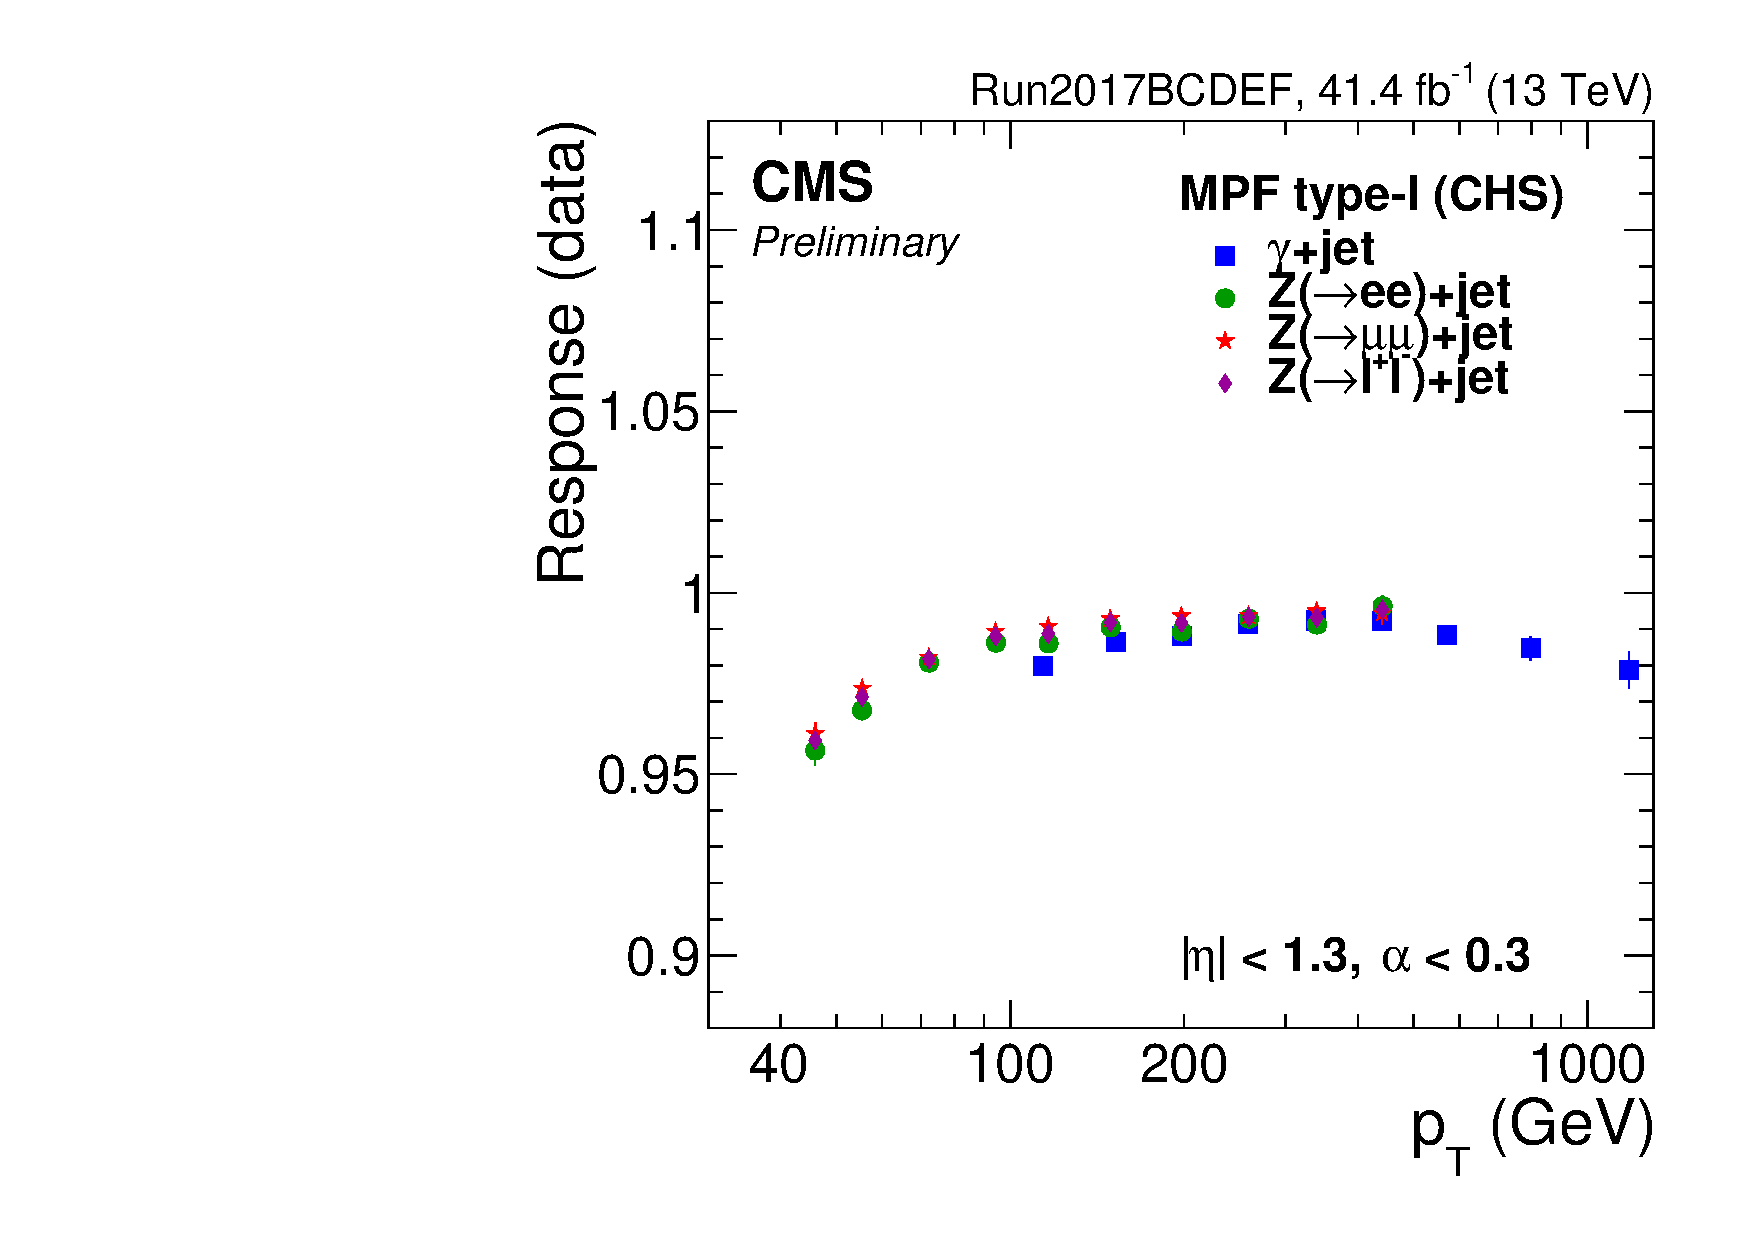
\includegraphics[width=0.32\textwidth]{BCDEF/paper_softrad_data_mpfchs1_vspt.pdf}
  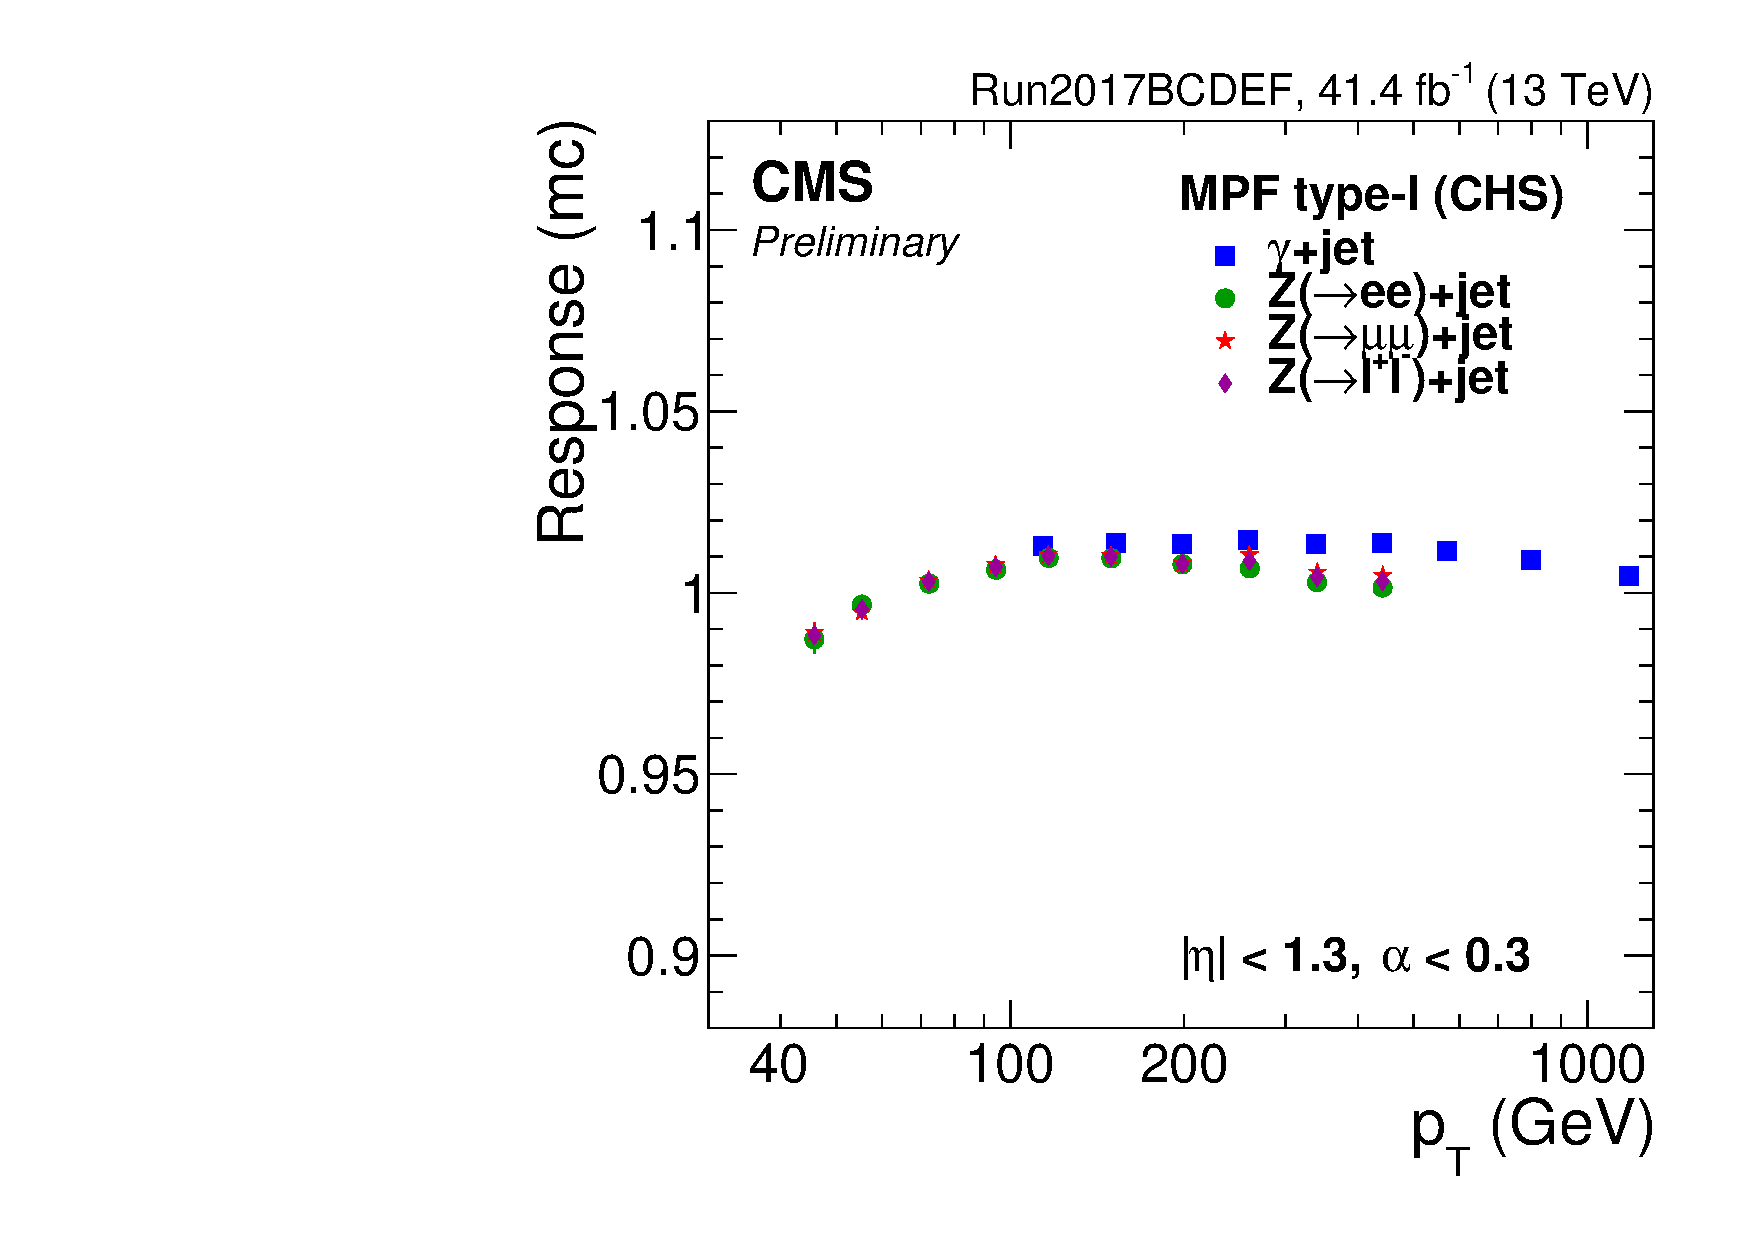
\includegraphics[width=0.32\textwidth]{BCDEF/paper_softrad_mc_mpfchs1_vspt.pdf}
  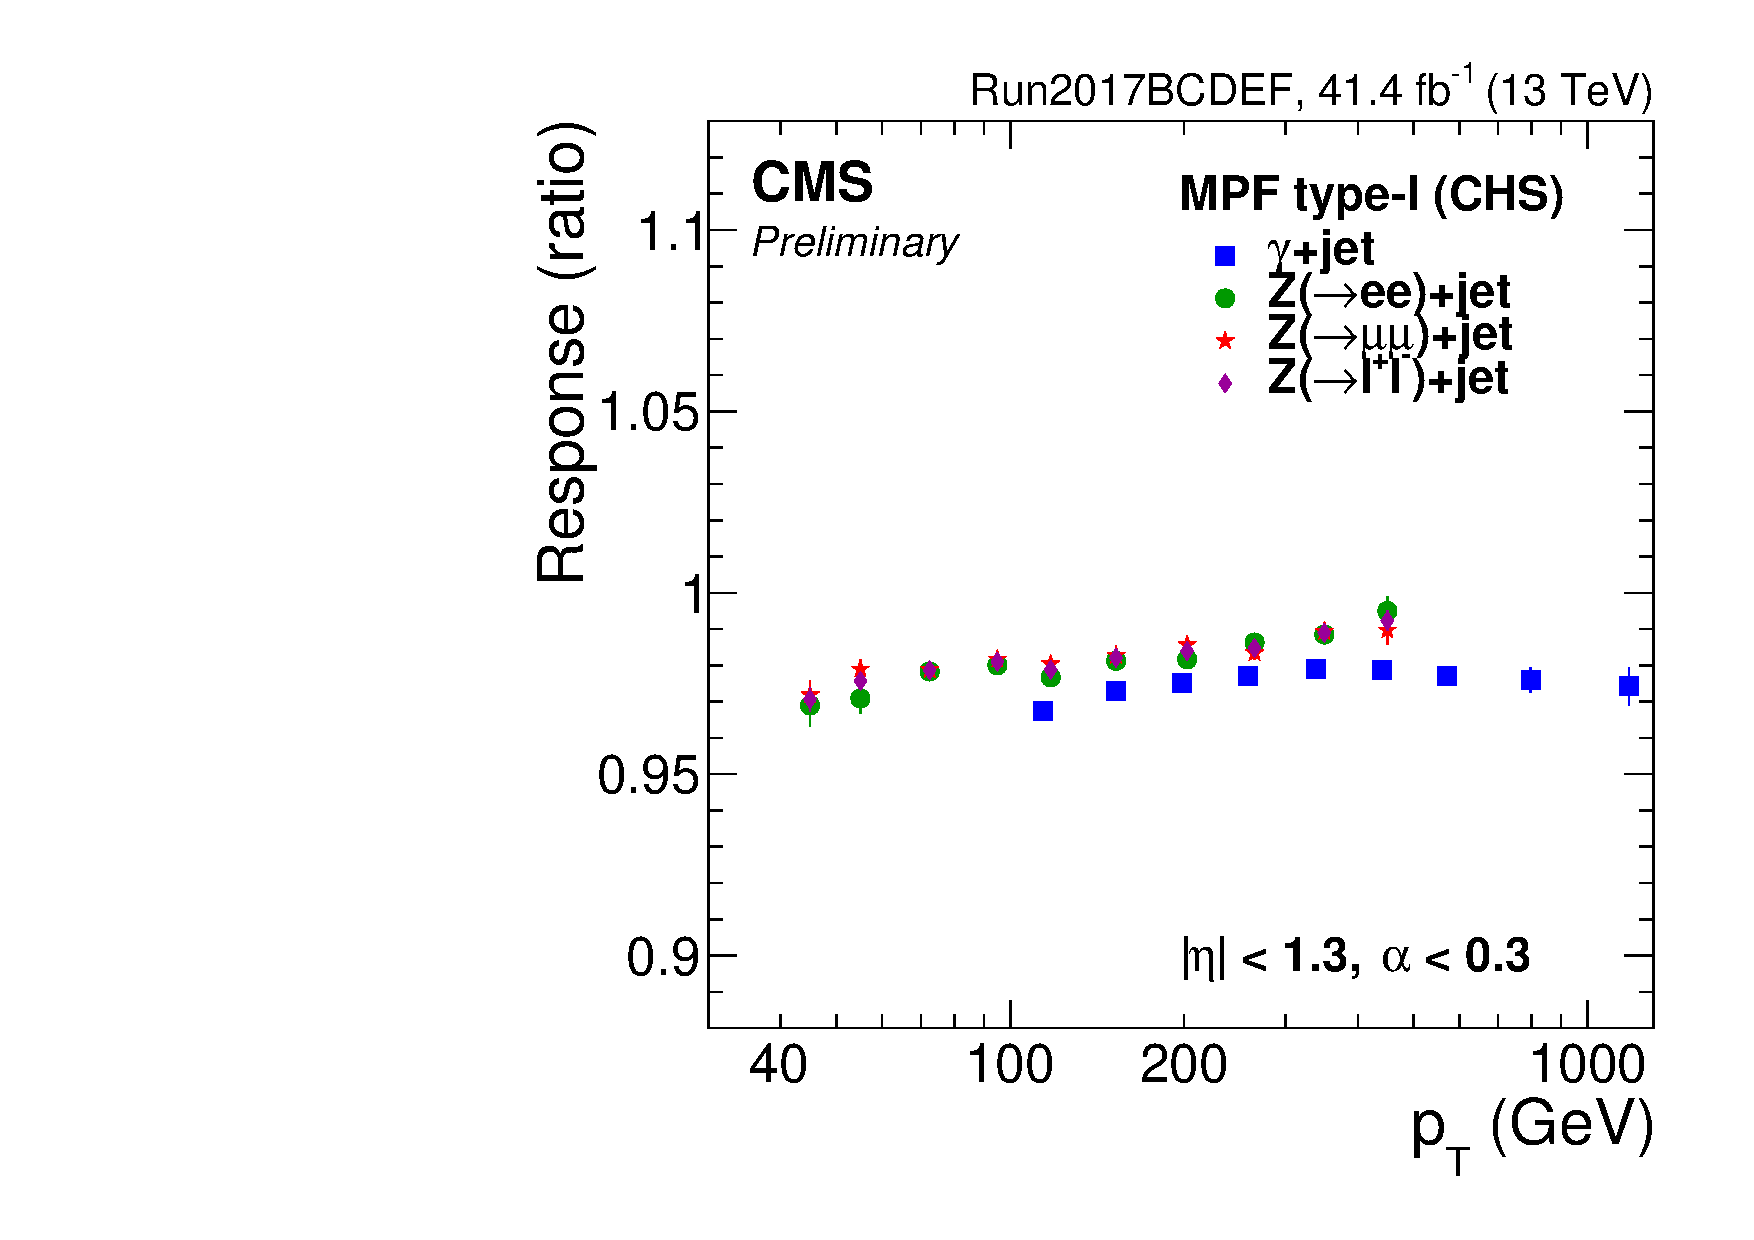
\includegraphics[width=0.32\textwidth]{BCDEF/paper_softrad_ratio_mpfchs1_vspt.pdf}\\
  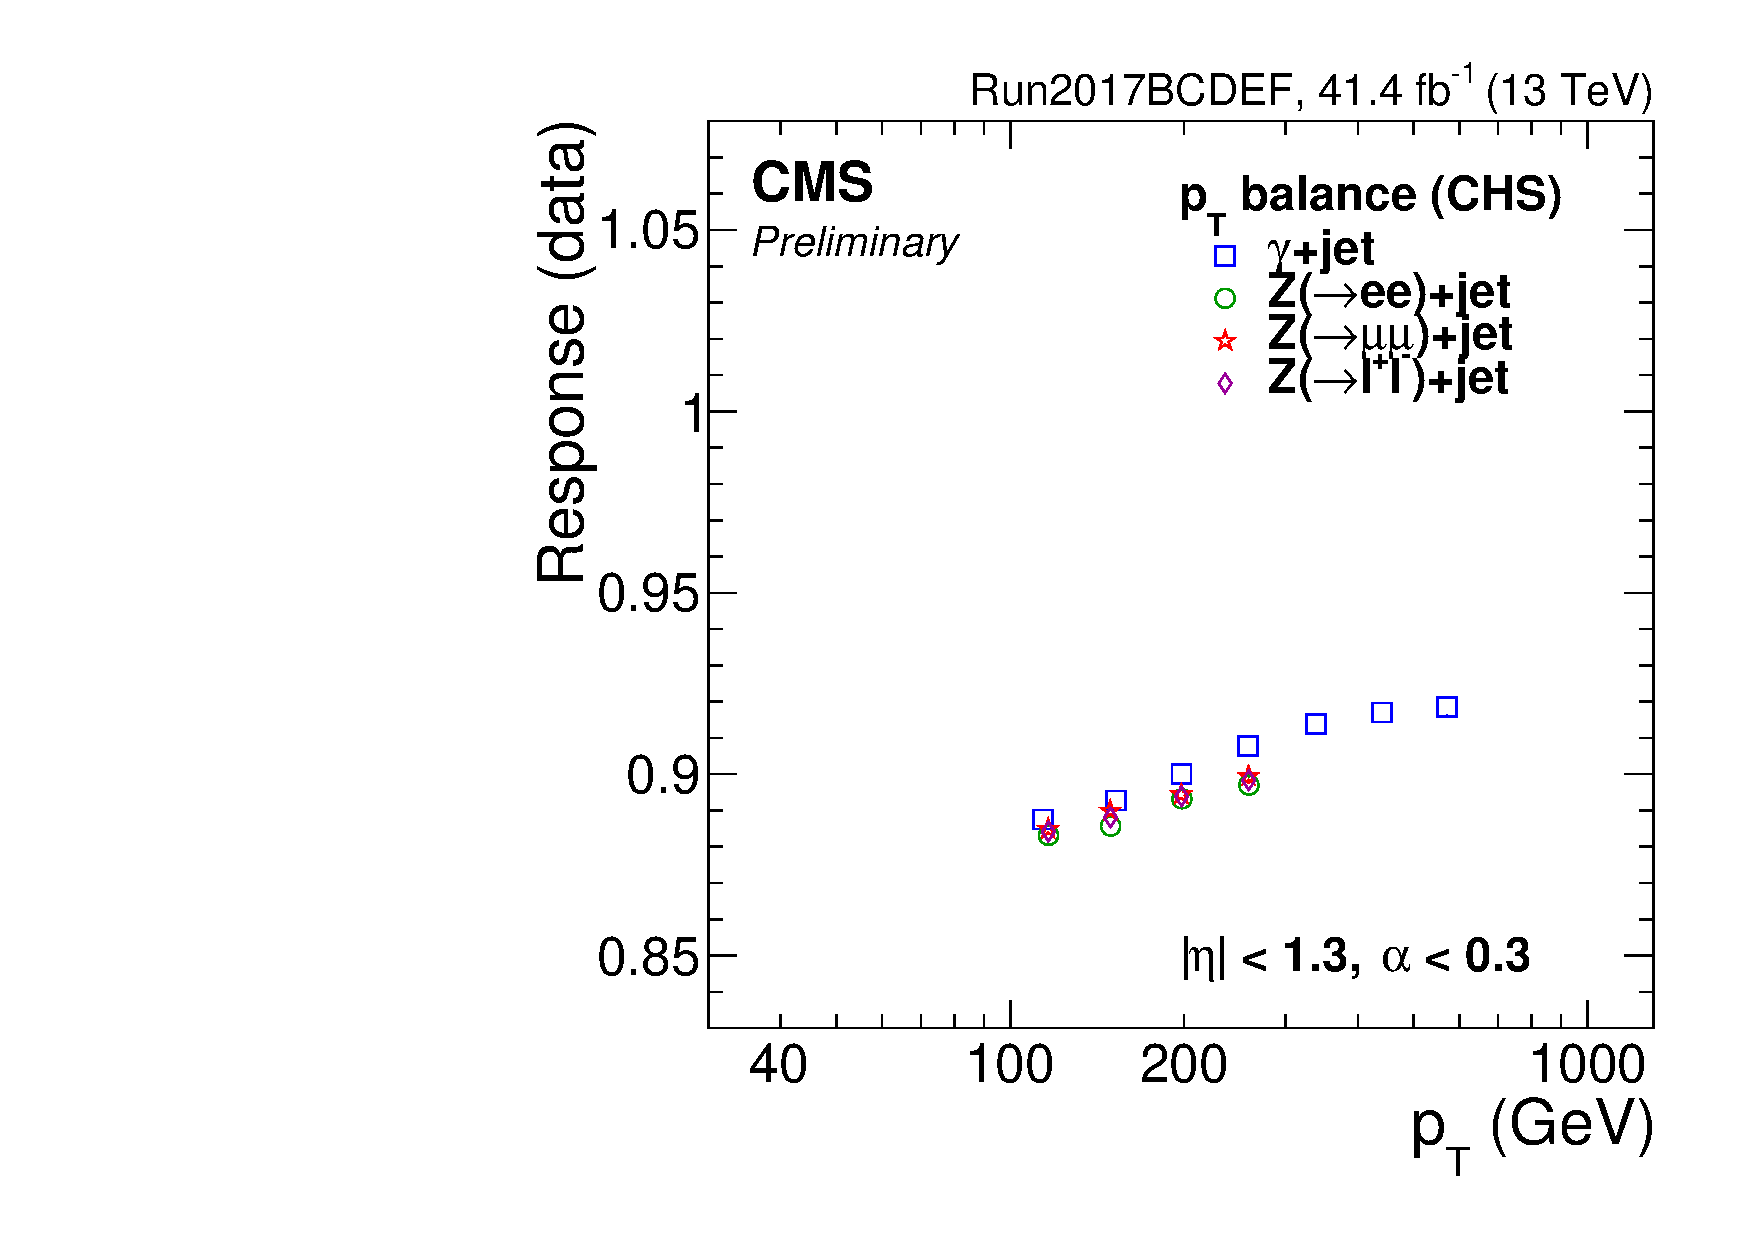
\includegraphics[width=0.32\textwidth]{BCDEF/paper_softrad_data_ptchs_vspt.pdf}
  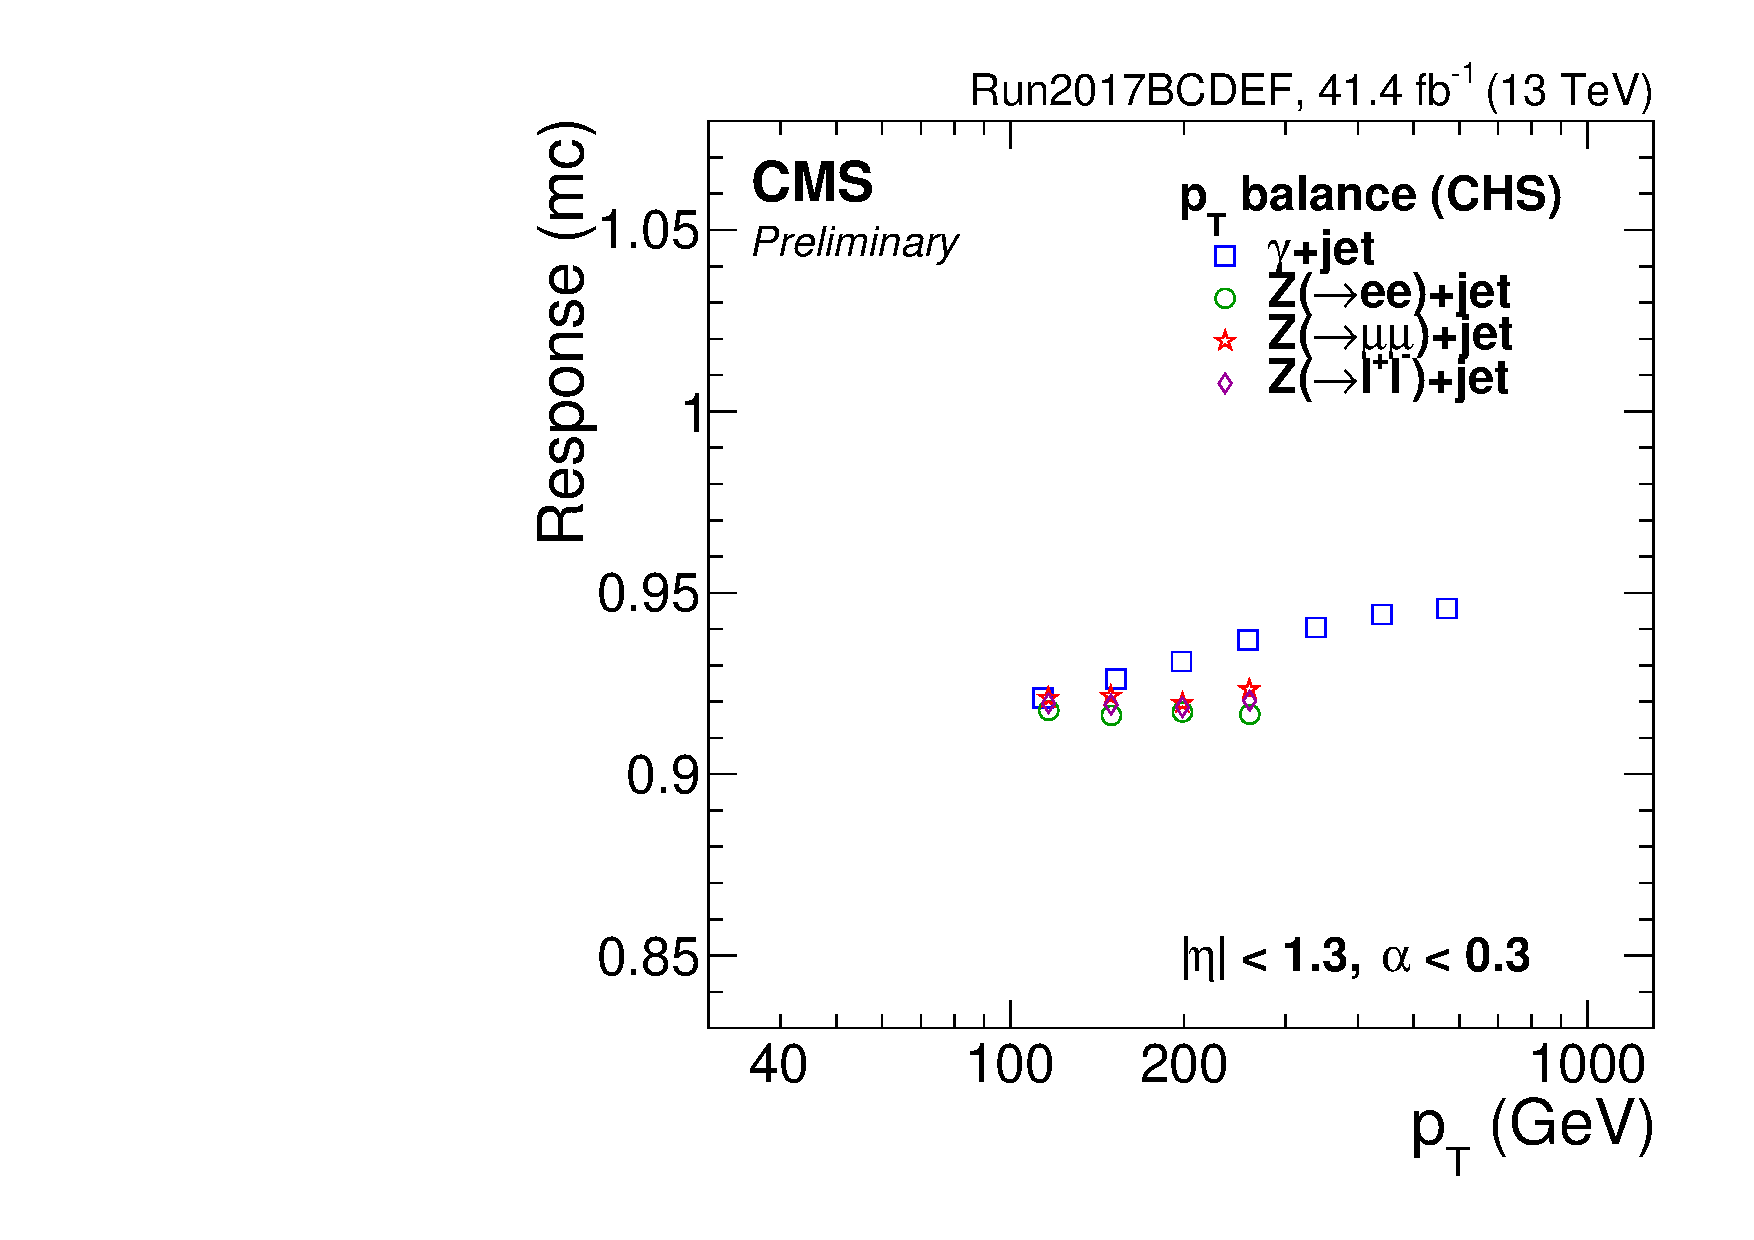
\includegraphics[width=0.32\textwidth]{BCDEF/paper_softrad_mc_ptchs_vspt.pdf}
  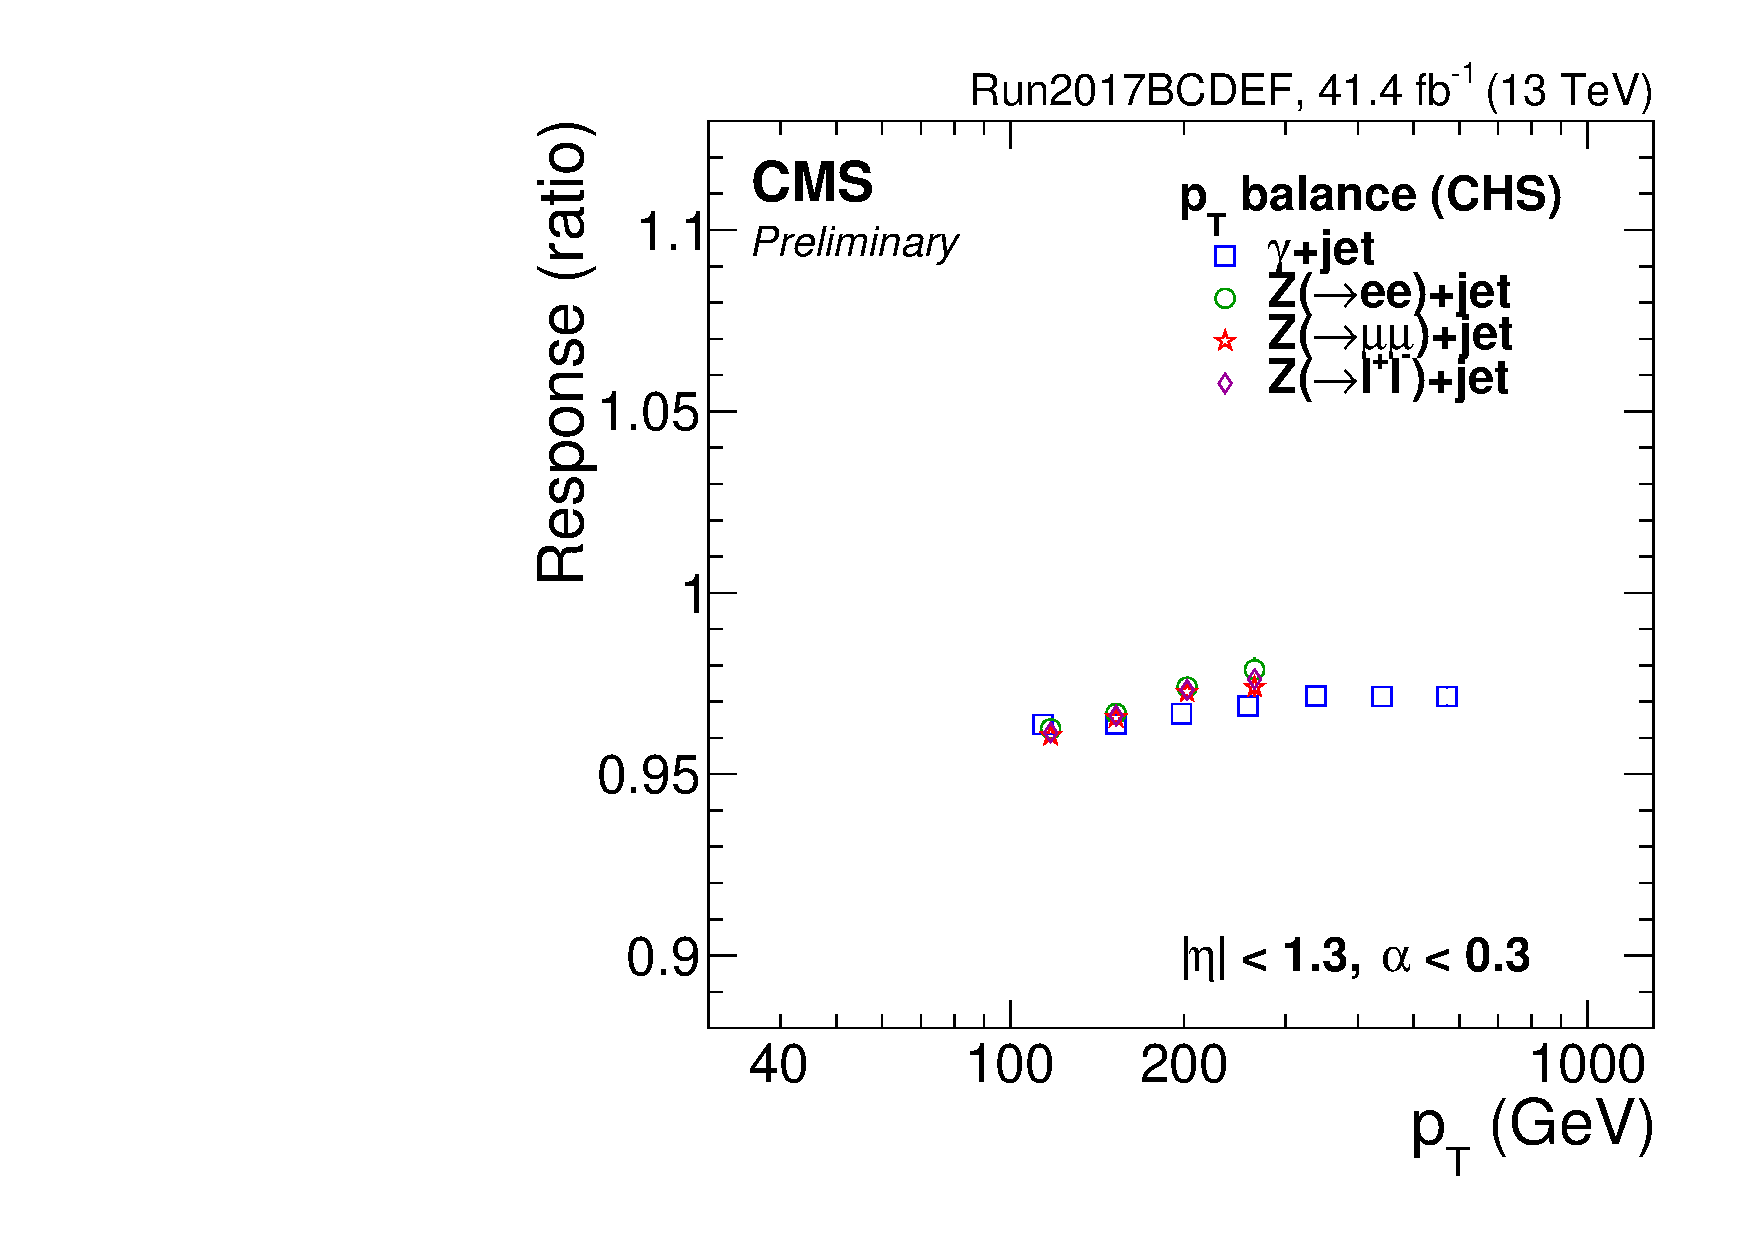
\includegraphics[width=0.32\textwidth]{BCDEF/paper_softrad_ratio_ptchs_vspt.pdf}\\
%  \includegraphics[width=0.32\textwidth]{drawEFvsGH_mpfchs1_ptchs_nogptb.pdf}
%  \includegraphics[width=0.32\textwidth]{drawBCDpEFvsGH_mpfchs1_ptchs_nogptb.pdf}
%  \includegraphics[width=0.32\textwidth]{drawBCDvsGH_mpfchs1_ptchs_nogptb.pdf}\\

%\foreach \n in \IOVs {
\foreach \n in {BCDEF,B,C,D,E,F} {
  \newpage
  \n \\
  \includegraphics[width=0.32\textwidth]{\n/globalFitL3res_raw.pdf}
  \includegraphics[width=0.32\textwidth]{\n/globalFitL3res_orig.pdf}
  \includegraphics[width=0.32\textwidth]{\n/globalFitL3res_shifted.pdf}\\
  \includegraphics[width=0.32\textwidth]{\n/globalFitL3res_hsrc.pdf}
  \includegraphics[width=0.32\textwidth]{\n/globalFitL3res_mpfchs1_kfsr.pdf}
  \includegraphics[width=0.32\textwidth]{\n/globalFitL3res_ptchs_kfsr.pdf}\\
}

\foreach \n in {BCDEF,B,C,D,E,F} {
  \newpage
  \n \\
  \includegraphics[width=0.32\textwidth]{\n/paper_softrad_data_mpfchs1_vspt.pdf}
  \includegraphics[width=0.32\textwidth]{\n/paper_softrad_mc_mpfchs1_vspt.pdf}
  \includegraphics[width=0.32\textwidth]{\n/paper_softrad_ratio_mpfchs1_vspt.pdf}\\
  \includegraphics[width=0.32\textwidth]{\n/paper_softrad_data_ptchs_vspt.pdf}
  \includegraphics[width=0.32\textwidth]{\n/paper_softrad_mc_ptchs_vspt.pdf}
  \includegraphics[width=0.32\textwidth]{\n/paper_softrad_ratio_ptchs_vspt.pdf}\\
}

\foreach \n in {BCDEF,B,C,D,E,F} {
  \newpage
  \n \\
 \includegraphics[width=1.00\textwidth]{\n/softrad_2x6_vspt_eta00-13.pdf}\\
}

\foreach \n in {BCDEF,B,C,D,E,F} {
  \newpage
  \n \\
  \includegraphics[width=0.32\textwidth]{\n/globalFitL3res_raw.pdf}
  \includegraphics[width=0.32\textwidth]{\n/globalFitL3res_orig.pdf}
  \includegraphics[width=0.32\textwidth]{\n/globalFitL3res_shifted.pdf}\\
  \includegraphics[width=0.32\textwidth]{\n/globalFitL3res_hsrc.pdf}
  \includegraphics[width=0.32\textwidth]{\n/globalFitL3res_mpfchs1_kfsr.pdf}
  \includegraphics[width=0.32\textwidth]{\n/globalFitL3res_ptchs_kfsr.pdf}\\

  \newpage
  \n \\
  \includegraphics[width=0.32\textwidth]{\n/paper_softrad_data_mpfchs1_vspt.pdf}
  \includegraphics[width=0.32\textwidth]{\n/paper_softrad_mc_mpfchs1_vspt.pdf}
  \includegraphics[width=0.32\textwidth]{\n/paper_softrad_ratio_mpfchs1_vspt.pdf}\\
  \includegraphics[width=0.32\textwidth]{\n/paper_softrad_data_ptchs_vspt.pdf}
  \includegraphics[width=0.32\textwidth]{\n/paper_softrad_mc_ptchs_vspt.pdf}
  \includegraphics[width=0.32\textwidth]{\n/paper_softrad_ratio_ptchs_vspt.pdf}\\

  \newpage
  \n \\
  \includegraphics[width=1.00\textwidth]{\n/softrad_2x6_vspt_eta00-13.pdf}\\

  \newpage
  \n \\
  \includegraphics[width=1.00\textwidth]{\n/softrad_2x6_kfsr_eta00-13.pdf}

}


\newpage


\end{document}
